\subsubsection{gSketch\cite{zhao_gsketch:_2011}}

\paragraph{}
gSketch is an extension of CountMin data structure. But unlike CountMin sketch, this is specifically geared towards summarizing graph streams. gSketch is based on one of the two assumptions that,

\begin{itemize}
    \item A graph stream sample is available.
    \item Both graph stream sample and a query workload sample are available.
\end{itemize}

\paragraph{}
As per the previous sketching technique, CountMin, a global sketch is created for the entire graph stream. The disadvantage of this method is that any structural properties present in the graph stream are completely ignored throughout this process. gSketch tries to avoid by considering the underlying structural properties of the graph.

\paragraph{}
The speciality of gSketch is to pre-process the stream samples and creating sketch partitions as indicated in \autoref{fig:gsketch}. Its goal is to maintain sufficient frequency uniformity within each localized sketch so that the query estimation can be optimized over the entire graph stream.

\begin{figure}[H]
    \centering 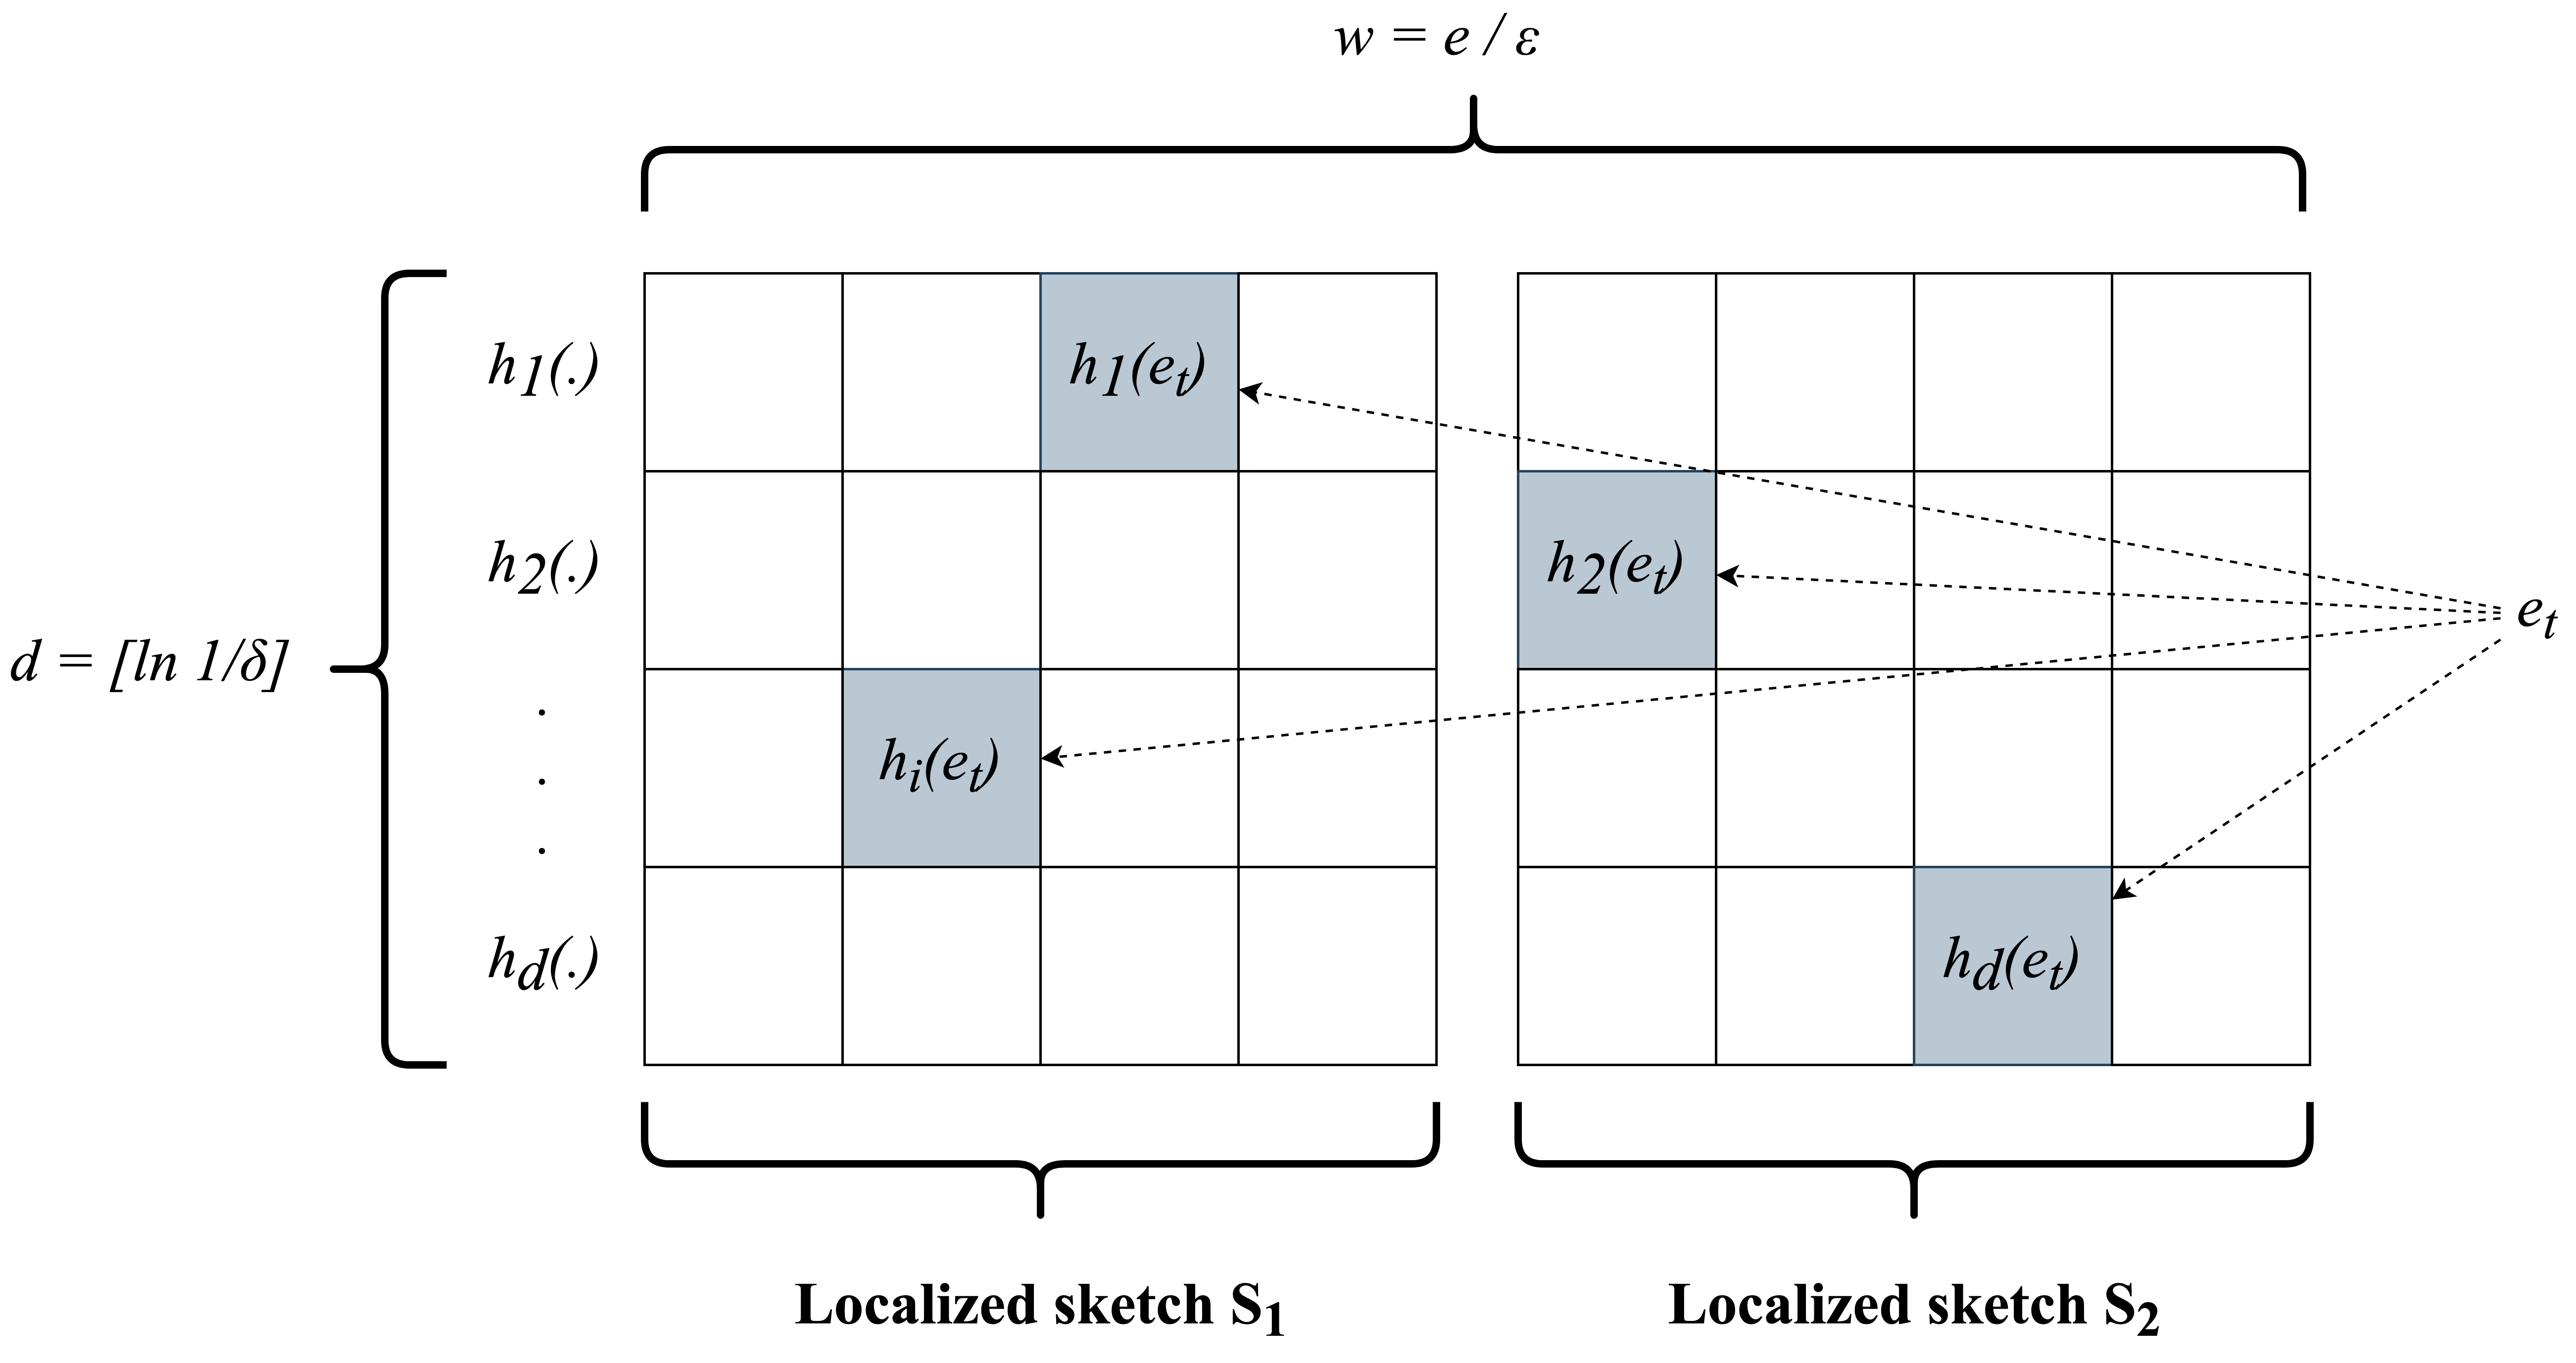
\includegraphics[width=\textwidth]{gsketch}
    \caption{gSketch sketch}
    \label{fig:gsketch}
\end{figure}